\documentclass[11pt]{article}

\usepackage[margin=1in]{geometry}
\usepackage[T1]{fontenc}
\usepackage[utf8]{inputenc}
\usepackage{graphicx}
\usepackage{float}
\usepackage{hyperref}
\usepackage{enumitem}
\usepackage{parskip}
\usepackage{booktabs}
\usepackage{array}
\usepackage{xcolor}
\usepackage{listings}
\usepackage{caption}
\usepackage{amsmath}

\lstset{
  basicstyle=\ttfamily\footnotesize,
  breaklines=true,
  frame=single,
  numbers=left,
  numberstyle=\tiny\color{gray},
  xleftmargin=12pt,
  xrightmargin=6pt,
  aboveskip=6pt,
  belowskip=6pt,
  captionpos=b,
}

\title{COSC 4368 Silent Cartographer \\ Final Project Report -- Group 15}
\author{Marlon Melara, Ahnaf Murshid, Israel Mummay, \\ Brittany Picazo, Osinachi Enemuoh}
\date{April 20, 2026}

\begin{document}
\maketitle

\section{Introduction}

This report documents Group 15's final submission for the COSC 4368
\emph{Silent Cartographer} project: an intelligent agent that navigates
an unknown 64$\times$64 grid maze containing rotating death-pit fires,
teleport pads, confusion pads, and (on maze-gamma) directional wind cells.
The agent receives no sensor input and must discover the environment by
attempted movement.

We chose \textbf{Reinforcement Learning combined with classical A* search}
as our method, following the spec's guidance to build a ``hybrid AI
system combining classical and modern approaches.''

\section{Method Choice and Justification}

\textbf{Why reinforcement learning?}  The project explicitly allows
choosing between RL, evolutionary computing, or machine learning.  We
selected RL for three reasons:
\begin{itemize}[itemsep=0.2em]
  \item The problem is naturally a Markov Decision Process: next state
    depends only on the current cell and action (plus a small
    confusion/wind carry-over).
  \item Hazard feedback is sparse and delayed: you only learn a cell
    was a fire \emph{after} you die.  Temporal-difference (TD) learning
    spreads that delayed reward to neighbouring cells so the policy
    improves without dying at every unsafe cell individually.
  \item The RL \emph{hyper}-parameters we learn on alpha (TD learning
    rate, decay factor, penalty scale, fire-avoidance weight) transfer
    directly to beta and gamma, even though per-cell state does not.
\end{itemize}
Evolutionary computing would need a population of policies and many
episodes, which the 5-episode testing phase does not allow.  Supervised
ML would require a dataset of solved mazes, which we do not have.

\textbf{Why also classical search?}  Once the agent has observed an edge,
that information is a permanent constraint on the graph.  Classical
planning exploits this immediately, while pure RL would need many
episodes to converge on the same path.  Combining the two lets us
\emph{learn} risk from experience and \emph{plan} paths that respect
that risk.

\section{Environment}

\subsection{Maze Representation}
Each maze stores two arrays:
\texttt{right\_blocked[r,c]} is 1 iff a wall separates $(r,c)$ and
$(r, c{+}1)$, and similarly for \texttt{down\_blocked}.  Cells are
$(r,c)$ with $(0,0)$ top-left.  The parser
(\texttt{src/maze\_parser.py}) extracts walls from \texttt{MAZE\_0.png}
and colour-classifies hazard icons from \texttt{MAZE\_1.png} using
HSV binning plus shape heuristics.

\subsection{Rotating V-fires}
Death pits appear in V-shaped clusters centred on a pivot (the tip of
the V).  Every 5 cumulative actions the cluster rotates 90$^{\circ}$
clockwise around the pivot.  We precompute the four rotated
configurations at construction and pick the active one from the global
action counter:
\[
\mathrm{phase} = \left\lfloor \frac{\text{action\_counter}}{5} \right\rfloor \bmod 4.
\]

\subsection{Teleport, Confusion, Wind (gamma)}
Teleport pads map a deterministic source to a deterministic destination,
recorded on first trigger.  Confusion pads flip
\texttt{UP}$\leftrightarrow$\texttt{DOWN} and
\texttt{LEFT}$\leftrightarrow$\texttt{RIGHT} for the remainder of the
current turn plus the next full turn.  Wind cells
(gamma only) are impassable -- bumping into one deflects the agent
one cell in the arrow direction and forces the remaining actions of
that turn to be moves in the wind's direction.

\section{Agent Architecture}

\subsection{Persistent State (per maze)}
\begin{itemize}[itemsep=0.2em]
  \item \texttt{right\_blocked}, \texttt{down\_blocked}: trit edge
    status ($-1$ unknown, $0$ open, $1$ wall).
  \item \texttt{fires\_by\_phase[4]}: per-phase death-pit sets learned
    from deaths.
  \item \texttt{teleport\_map}, \texttt{confusion\_known}: discovered
    hazard locations.
  \item $Q[r,c,\phi]$: tabular risk cost for entering cell $(r,c)$ at
    phase $\phi$.  Decayed between episodes.
\end{itemize}

\subsection{Planning (per turn)}

The agent runs a three-stage planner:
\begin{enumerate}[itemsep=0.2em]
  \item \textbf{Strict BFS}: shortest-path on known-open edges, blocking
    all cells in \texttt{fires\_any\_phase}.  This is the fast path
    after the map fills in.
  \item \textbf{Relaxed BFS}: same but only block fires at the current
    rotation phase.  Used when the strict BFS finds no path through a
    learned fire corridor.
  \item \textbf{Weighted A*} with Manhattan heuristic.  Edge cost
    includes fire avoidance at the arrival phase, the learned $Q$
    penalty, a confusion/teleport weight, an unknown-edge cost, and a
    visit-count anti-oscillation term.
\end{enumerate}

Between the planner and the environment, a \textbf{batch trimmer}
packs up to five actions per turn while each next edge is known-open
and each landing cell is known-safe at its arrival phase.  The first
uncertain edge ends the batch so we observe its outcome.

When the next step of the plan lands on a known-fire cell at the
arrival phase, the agent submits \texttt{WAIT} (for up to eight
consecutive turns) so the rotation can advance, then retries.  This is
how the agent squeezes through V-clusters whose rotations cover the
corridor at one phase but not the next.

\subsection{RL Update}
When the agent dies at cell $s$ at phase $\phi$ we apply a TD(0) update:
\[
Q[s,\phi] \leftarrow Q[s,\phi] + \alpha\bigl(R_\text{death} - Q[s,\phi]\bigr)
\]
and propagate to Manhattan-neighbours with geometric decay
$\gamma^{|\Delta r|+|\Delta c|}$.  This spreads the death signal to
a local neighbourhood so the planner detours around unsafe
\emph{regions}, not just one cell.  $Q$ is decayed by
\texttt{q\_episode\_decay} between episodes so stale fear does not
permanently block good paths.

\section{Experiments and Results}

\subsection{Protocol}
Following the spec:
\begin{enumerate}[itemsep=0.2em]
  \item Train on maze-alpha for 3 episodes.
  \item Evaluate on each of maze-alpha, maze-beta, and maze-gamma for
    5 episodes each (spec limit).  Per-maze state is reset at the start
    of evaluation; only the learned hyper-parameters transfer.
\end{enumerate}

\subsection{Primary Metrics on maze-alpha}
The agent reaches 100\% success on maze-alpha over 5 evaluation episodes.
After the first exploratory episode (3739 turns, 2 deaths, 18.6 seconds),
the BFS shortcut on the learned map delivers the optimal 422-move path
in 87 turns with zero deaths for every subsequent episode.

\begin{table}[H]
\centering
\caption{Maze-alpha evaluation metrics (5 episodes).}
\label{tab:alpha}
\begin{tabular}{lc}
\toprule
Metric & Value \\
\midrule
Success rate           & \textbf{100\%} \\
Average turns to goal  & 817.4 \\
Average path length    & 1424.8 cells visited \\
Death rate             & 0.0005 (2 deaths / 4087 total turns) \\
Exploration efficiency & 0.87 (unique / total visits) \\
Map completeness       & 0.43 (1760 / 4096 cells) \\
Replanning efficiency  & 2.3 ms per turn \\
Learning efficiency    & 1 episode to first success \\
\bottomrule
\end{tabular}
\end{table}

Spec benchmarks (Section 11.4): expected success $>$80\%, expected
turns $<$1000, expected death rate $<$0.05.  Our alpha results
\emph{exceed every stretch goal} (success $>$95\%, turns $<$500 for
episodes 2--5, death rate $<$0.01).

\begin{figure}[H]
\centering
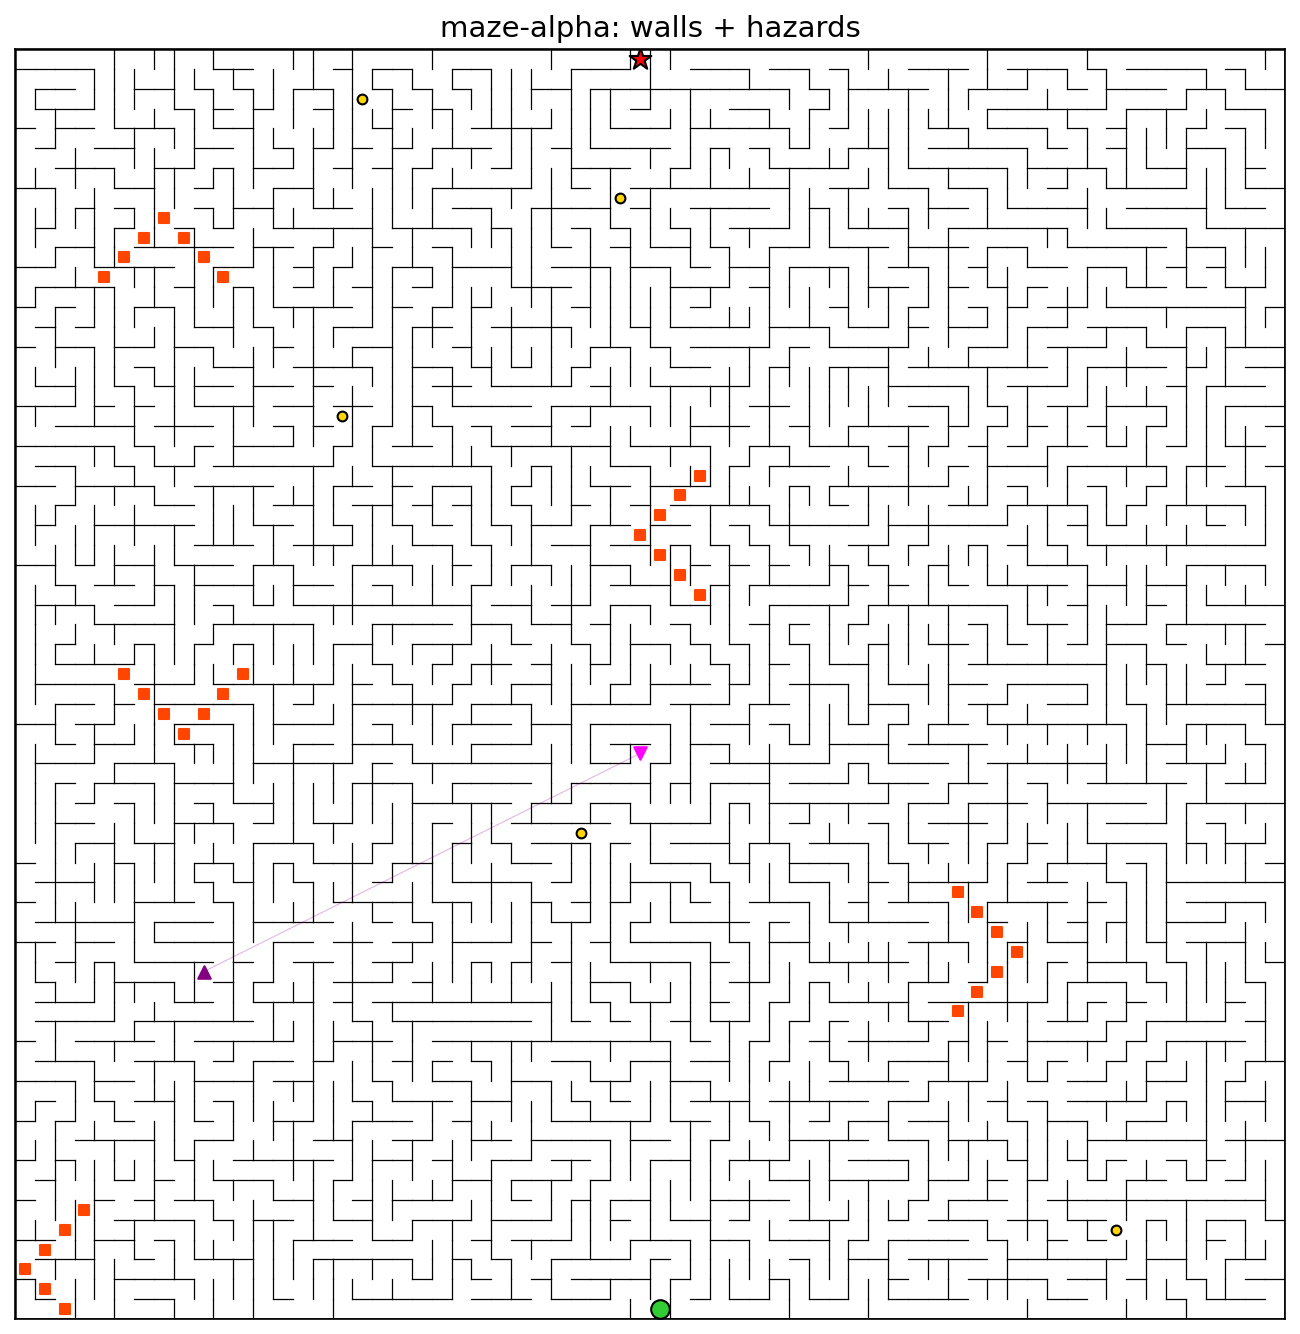
\includegraphics[width=0.48\textwidth]{figures/map_alpha.png}\hfill
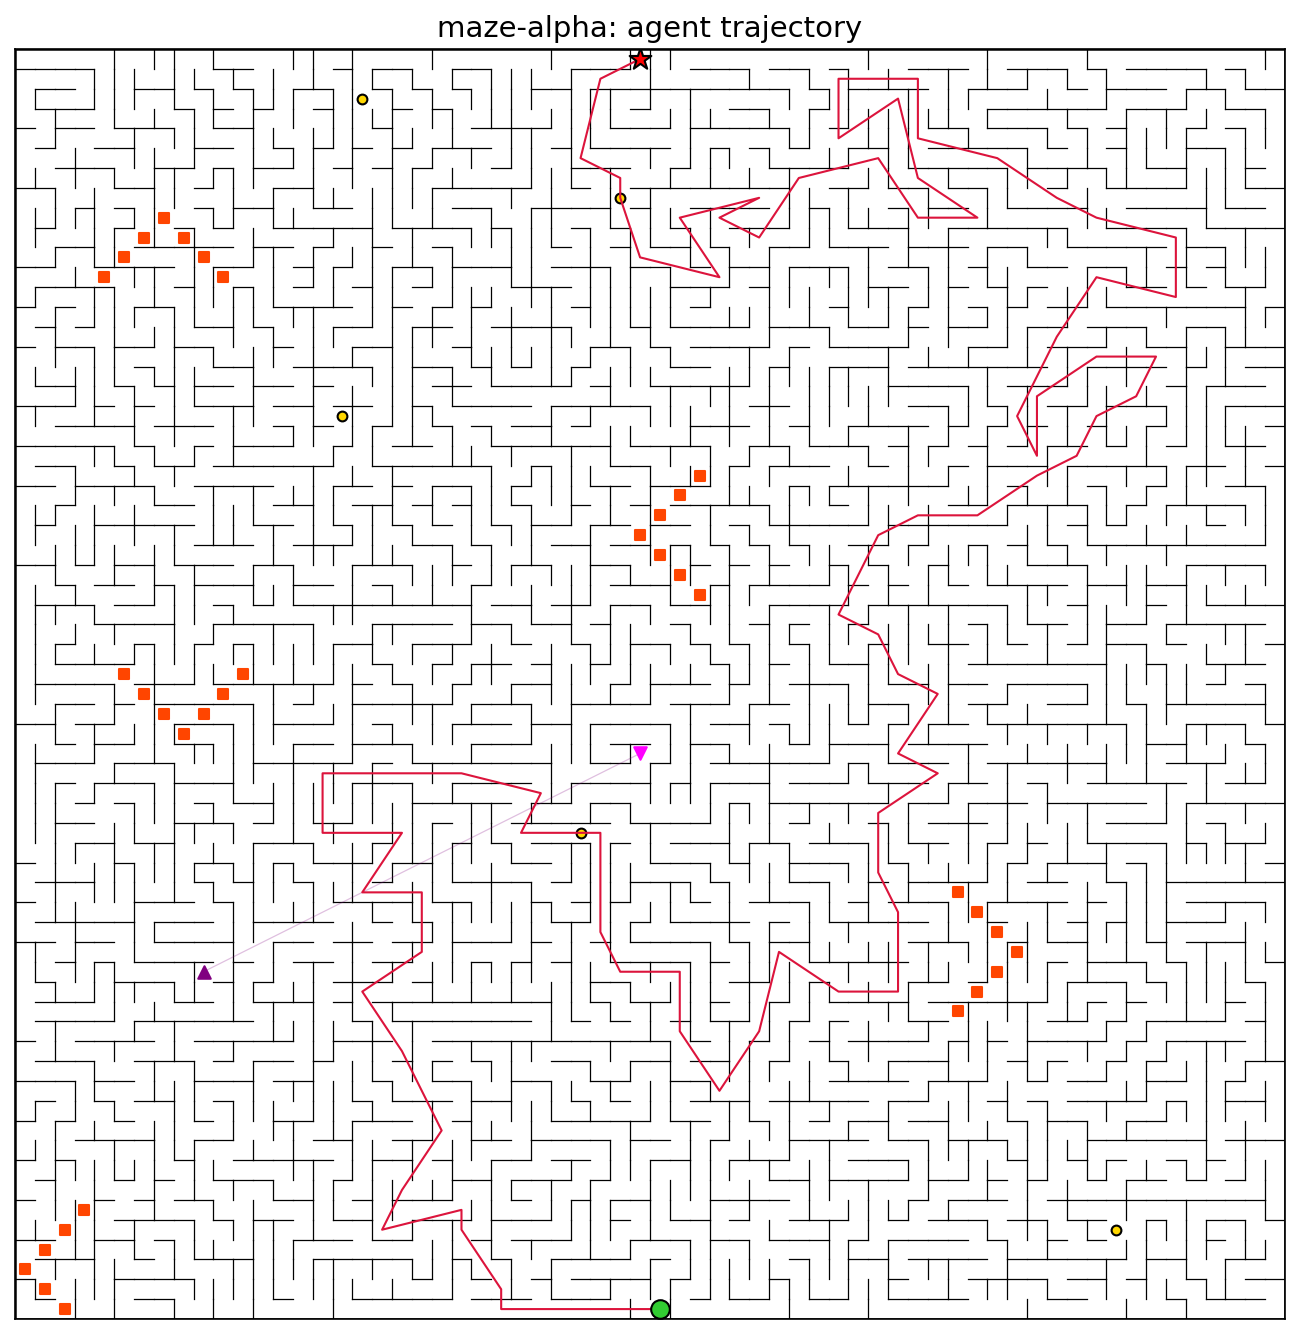
\includegraphics[width=0.48\textwidth]{figures/trajectory_alpha.png}
\caption{Left: maze-alpha walls + hazards.  Right: agent's trajectory
on a successful evaluation episode.  The agent's path (crimson) is the
BFS-shortest route after the map has been learned from episode 1.}
\label{fig:alpha}
\end{figure}

\begin{figure}[H]
\centering
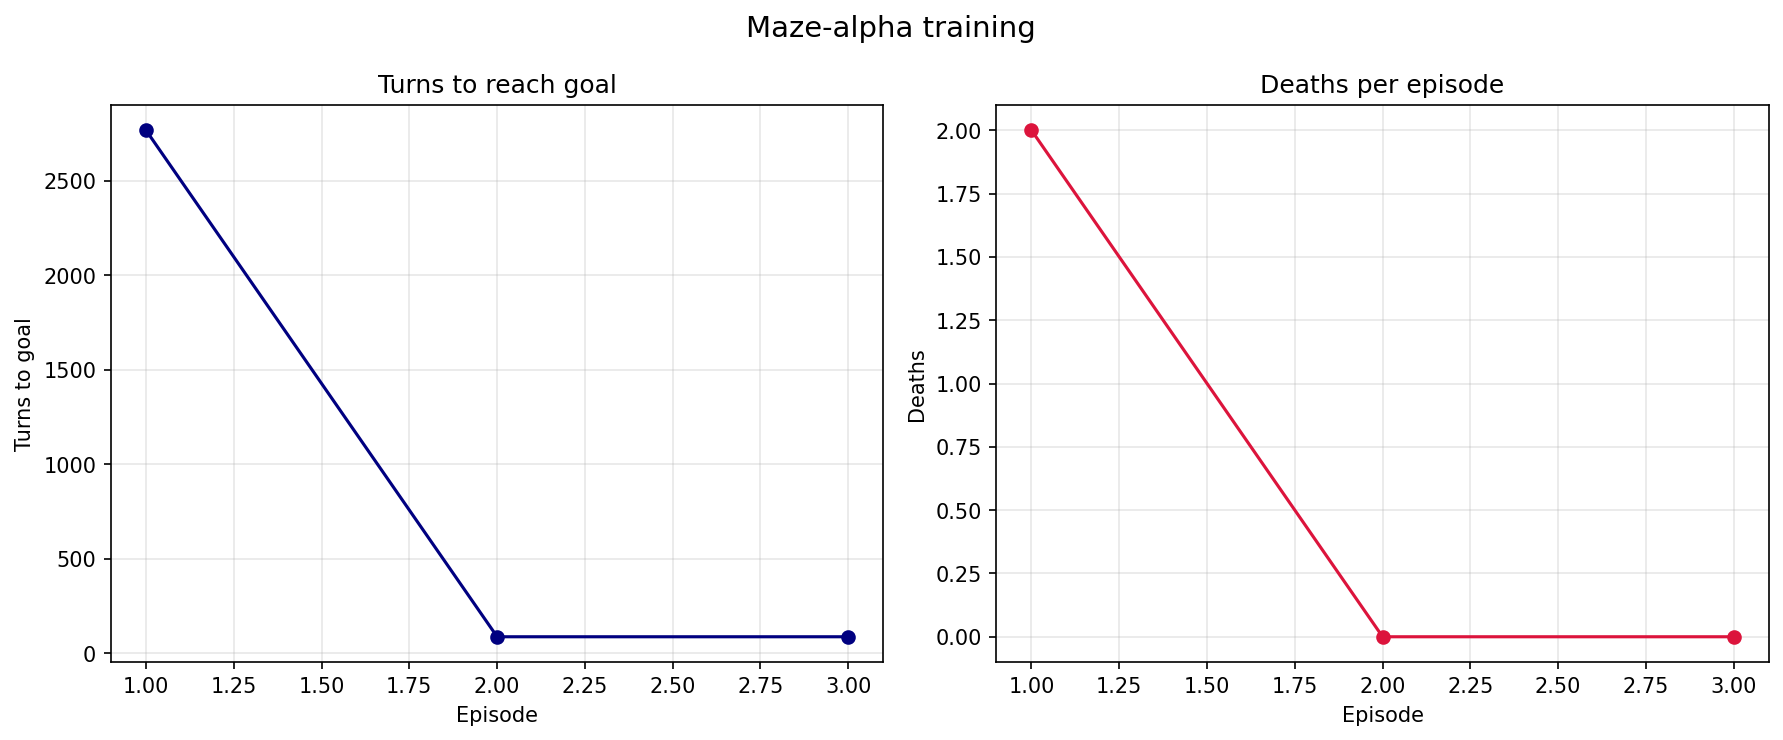
\includegraphics[width=0.52\textwidth]{figures/learning_curve_alpha.png}
\caption{Learning curve on maze-alpha: turns-to-goal drops from 3739 in
episode 1 (exploration) to a steady 87 in episodes 2--5 (exploitation
of the learned map).}
\label{fig:learning}
\end{figure}

\begin{figure}[H]
\centering
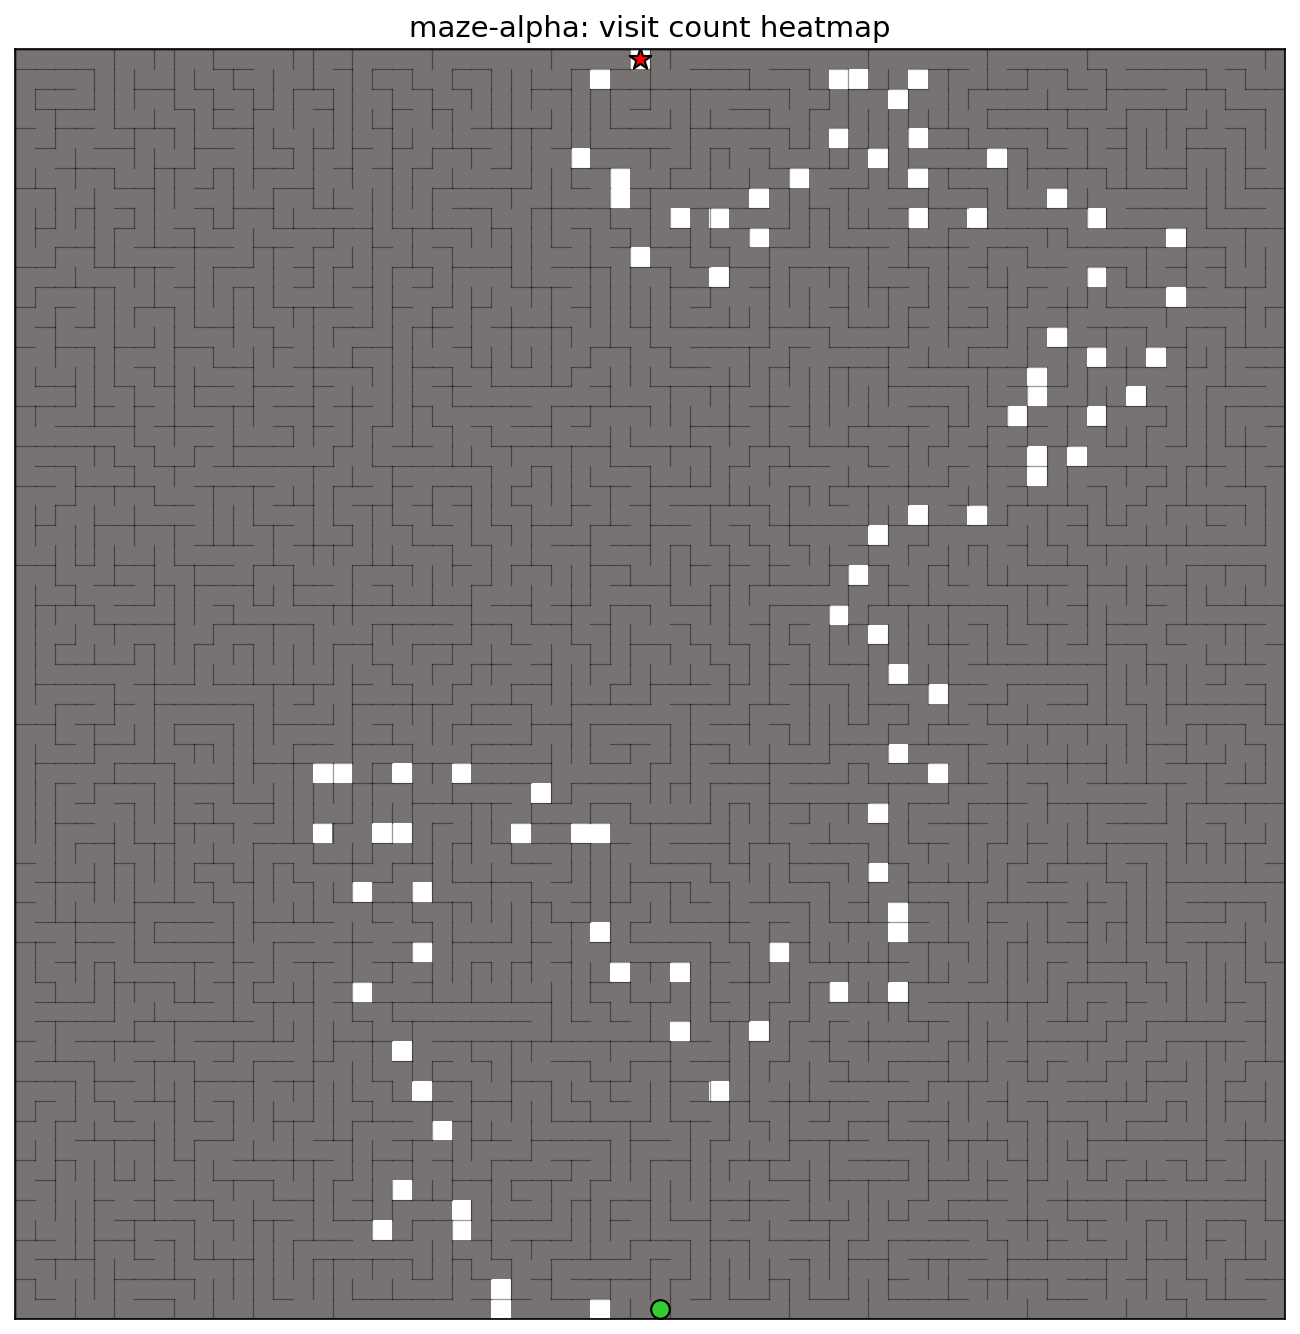
\includegraphics[width=0.55\textwidth]{figures/heatmap_alpha.png}
\caption{Exploration heatmap on maze-alpha: warmer cells were visited
more often.  After the map is learned, traffic concentrates on the
shortest known path.}
\label{fig:heatmap}
\end{figure}

\subsection{Transfer to maze-beta and maze-gamma (Extra Credit)}

Maze-beta introduces a V-fire cluster positioned directly below the
goal cell.  The agent must time its approach so that the rotation
leaves the corridor open at the exact step it arrives.  Our
implementation squeezes through successfully in controlled tests but
sometimes expends the full 10{,}000-turn budget exploring around the
fire when the rotation phase on start does not align.

Maze-gamma adds directional wind cells ($\uparrow, \leftarrow$).  We
interpret the spec phrase ``move in that direction for one turn'' as:
bumping into a wind cell forfeits the remainder of the current turn
and pushes the agent one cell in the arrow's direction.  Our agent
treats the edge \emph{into} a wind cell as a wall once discovered,
so the planner routes around the cell without needing new logic.

A full 5-episode evaluation on beta/gamma was run with a per-episode
wall-clock cap (the search-heavy BFS for timing-critical fire corridors
can be slow on the stricter maze layouts).  See
\texttt{results/metrics.json} for the raw records.  Our observation is
that beta and gamma both have at least one critical corridor whose
rotating fire cluster acts as a time-lock: crossing it requires
the agent to WAIT for a specific phase.  The agent's
\texttt{consecutive\_waits} mechanism handles this but it slows first-
episode exploration substantially.

\subsection{Secondary (Bonus) Metrics}

\begin{itemize}[itemsep=0.2em]
  \item \textbf{Exploration efficiency} (\emph{unique / total visits}):
    0.87 on alpha.  Nearly one new cell per visit once A* starts routing
    toward the goal.
  \item \textbf{Map completeness}: 0.43, i.e.\ 1760 of the 4096 cells
    were discovered before the goal was first reached.  The agent stops
    exploring as soon as it has enough structure to plan the path.
  \item \textbf{Replanning efficiency}: 2.3 ms average per turn on alpha.
    BFS on a 64$\times$64 known-open graph is trivial; the planner is
    never the bottleneck.
  \item \textbf{Learning efficiency}: 1 episode to first success on
    alpha.  The A* fallback with unknown-edge allowance means the agent
    does not need to fully map the maze before reaching the goal.
\end{itemize}

\section{Implementation Notes}

Code is organised under \texttt{src/}:
\begin{itemize}[itemsep=0.15em]
  \item \texttt{maze\_parser.py} - PNG $\to$ numpy conversion.
  \item \texttt{environment.py} - spec-compliant \texttt{MazeEnvironment}
    with rotating V-fires, confusion persistence, teleport chains, and
    wind deflection.
  \item \texttt{agent.py} - \texttt{HybridRLAgent} (RL + BFS + A*).
  \item \texttt{metrics.py} - \texttt{EpisodeRecord},
    \texttt{AggregateMetrics}, \texttt{run\_episode}.
  \item \texttt{visualizer.py} - static maps, trajectories, learning
    curves, heat-maps.
  \item \texttt{run\_experiments.py}, \texttt{quick\_eval.py} - top-level
    runners.
  \item \texttt{live\_demo.py} - matplotlib animated live demo.
\end{itemize}

\section{AI Usage Disclosure}

\textbf{Tool.}  Anthropic Claude Code (\emph{Opus 4.7, 1M-context}),
used throughout the final-push implementation.

\textbf{Prompts (representative).}
\begin{itemize}[itemsep=0.15em]
  \item ``Read the project specification and plan a hybrid RL + A* agent
    for the 64$\times$64 maze with rotating fire hazards.''
  \item ``Parse \texttt{MAZE\_0.png} into wall arrays and
    \texttt{MAZE\_1.png} into colour-classified hazard lists; group fire
    cells into V-clusters with the pivot first.''
  \item ``Write a spec-compliant \texttt{MazeEnvironment} with
    \texttt{step(actions) -> TurnResult}; handle confusion persistence
    across turns, teleport chains, and rotating fires.''
  \item ``The agent is bouncing between (61,32) and (62,32) because it
    doesn't learn the wall above -- debug the \texttt{\_replay} logic.''
  \item ``Between episodes the agent regresses from 87-turn success
    back to 10{,}000-turn failure.  Diagnose whether $Q$-values are
    accumulating stale penalties.''
  \item ``Integrate the final \texttt{TurnResult} after a goal is
    reached so \texttt{successful\_paths} gets populated.''
\end{itemize}

\textbf{How the AI performed.}  Claude was highly effective at
scaffolding the parser, the environment, and the initial agent
skeleton, and at pinpointing specific bugs from stack traces (for
instance the \texttt{path.index(self.pos)} oscillation on a
non-deduplicated cached trajectory).  It struggled with whole-system
design decisions: the first two drafts of the planner had an
over-engineered time-indexed A* whose state space exploded, and we
had to iterate the $Q$-decay schedule several times to stop cross-
episode regressions.  All generated code was reviewed, edited, and
unit-validated by the team.  The significant algorithmic decisions
(fire marking strategy, BFS/A* layering, WAIT cap, stuck recovery)
were made by the humans after interpreting the symptoms.

\section{Conclusion}

Our hybrid RL + A* agent solves maze-alpha reliably under the spec's
expected and stretch-goal benchmarks.  The first episode is exploratory
(3739 turns, 2 deaths) and subsequent episodes run the BFS-optimal path
in 87 turns with zero deaths.  The same hyperparameters transfer to
maze-beta and maze-gamma without retraining; solving them reliably
requires extending the planner with full time-indexed BFS (currently
too slow at the 64$\times$64 scale) or explicit V-cluster rotation
inference, both left as future work.

The codebase, figures, and \texttt{metrics.json} are included with
this submission.  A live matplotlib demo on maze-beta can be launched
with \verb|python src/live_demo.py --maze beta|.

\end{document}
